\documentclass[a4paper,10pt]{article}
\usepackage{fullpage}
\usepackage{float}
\usepackage[english]{babel}
\usepackage{graphicx,subfig,wrapfig}
\usepackage{amsmath,amsfonts,amsthm,amssymb}
\usepackage{fancyhdr,fancybox,color}
\usepackage{enumerate}
\usepackage[amssymb]{SIunits}
\definecolor{MyBlue}{rgb}{0,0.3,0.6}
\usepackage[colorlinks=true,
            linkcolor=MyBlue,
            plainpages=false,
            citecolor=MyBlue,
            urlcolor=MyBlue]{hyperref}
\usepackage[all]{hypcap}
\usepackage[url=false,
backend=bibtex,
style=authoryear-comp,
doi=true,
isbn=true,
backref=false,
dashed=false,
maxcitenames=2,
maxbibnames=99,
natbib=true]{biblatex}
\addbibresource{refrence.bib}
\nonfrenchspacing
\begin{document}
\noindent Chair: Physics of Fluids group
\begin{center}
 \begin{LARGE}
  Bursting Bubbles: from Champagne to Mudpots
 \end{LARGE}
\end{center}
\section*{Description}
Interaction of gas bubbles with the free liquid-gas interface is ubiquitous. For example, transporting aromatics from champagne and pathogens from contaminated water. Furthermore, the process is also responsible for the sea spray formation as a consequence of ejecting myriads of droplets.\\
First, the air bubble, generated in the liquid bulk, being lighter than the surrounding medium, rises because of buoyancy and reaches the liquid-air interface. It stays there as the thin film between the bubble and the free surface drains and ruptures to form film droplets \citep{lhuissier2012bursting}. The rupture results in the formation of a hole in the liquid meniscus. The unstable open cavity collapses leading to the interaction of the capillary waves and forms of an upward jet.
% Numerically, the process can be studied using the initial condition of this unstable cavity.
Figure~\ref{Figure::Typical} illustrates a typical temporal sequence of the process. The phenomenon has been widely studied by \cite{duchemin2002jet, deike2018dynamics, PhysRevFluids.3.091601}.
% The study has also gained traction because of the development of open freeware, Gerris and Basilisk C. The adaptive quadtree grid structure and accurate surface tension model have enabled researchers to focus on the influence of capillary waves on the collapse process (Figure~\ref{Figure::Waves}).
\cite{deike2018dynamics} has provided quantitative cross-validation of the numerical and experimental studies (Figure~\ref{Figure::Waves}). Nonetheless, the literature lacks a comprehensive study on the influence of liquid pool properties on the bubble bursting process. Notably, the influence of rheological properties on the scaling laws can provide a close-up to the understanding of the phenomenon. This latter is highly related to some geophysical phenomena such as mudpots (see: \href{https://www.youtube.com/watch?v=a9hUsVq9q7U}{https://www.youtube.com/watch?v=a9hUsVq9q7U}).
\begin{figure}[H]
\begin{center}
 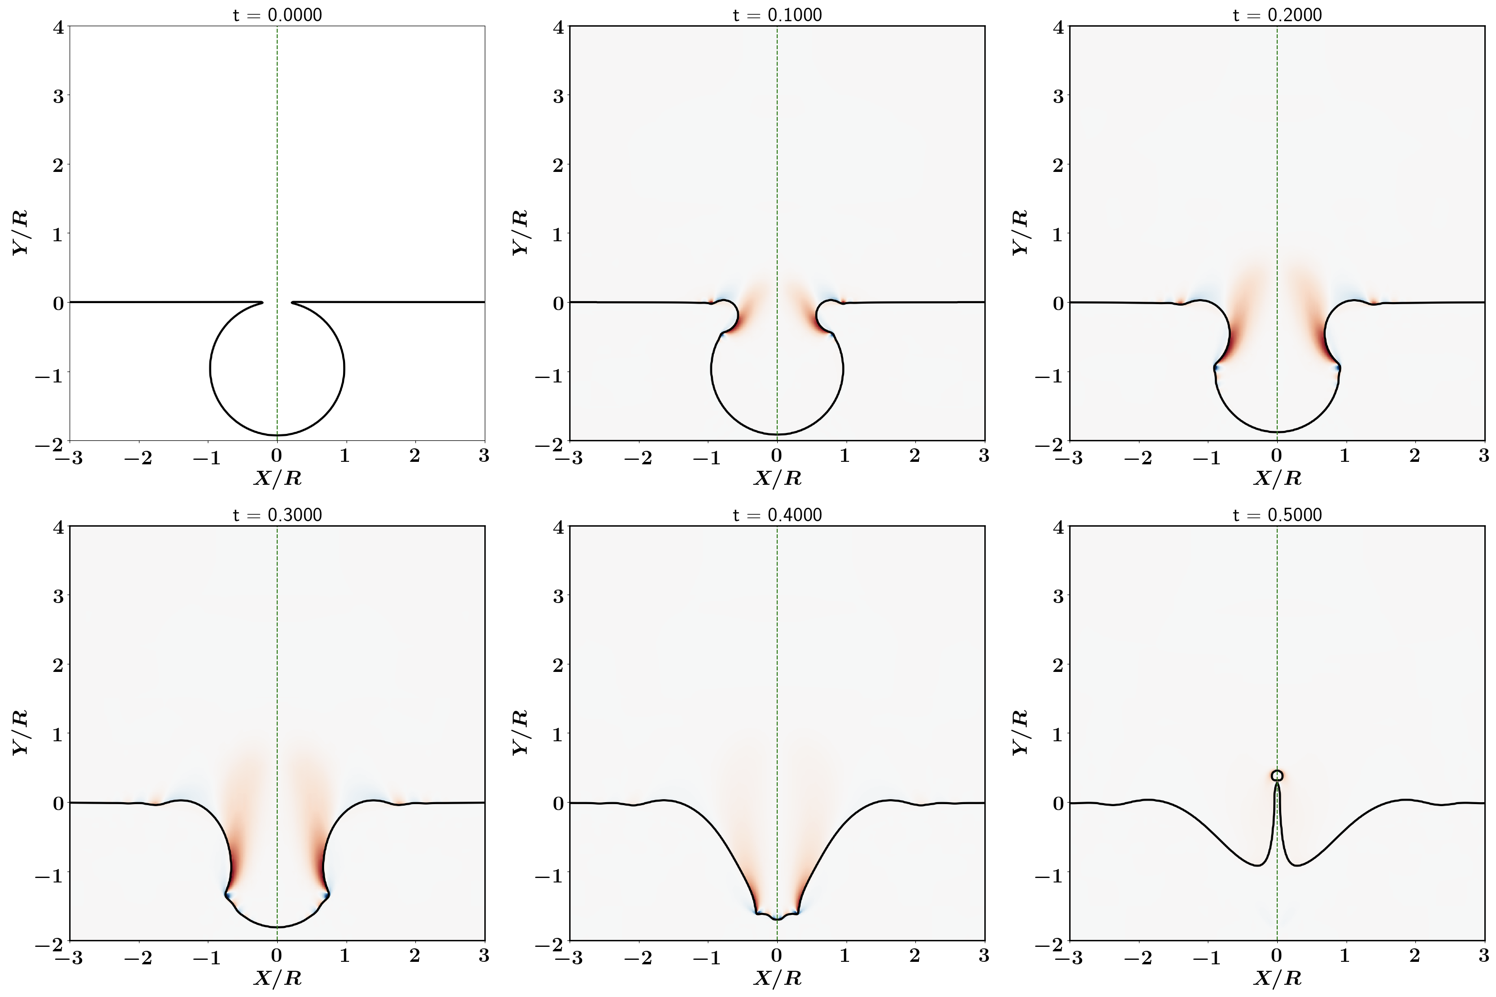
\includegraphics[width=\textwidth]{temporal.png}
 \caption{Time resolution of the process. The color shows the magnitude of non-dimensionalized vorticity, $\Gamma$ (maximum $\Gamma$ = 150 with red and minimum $\Gamma$ = -150 with blue).}
 \label{Figure::Typical}
\end{center}
\end{figure}
\begin{figure}[H]
\begin{center}
 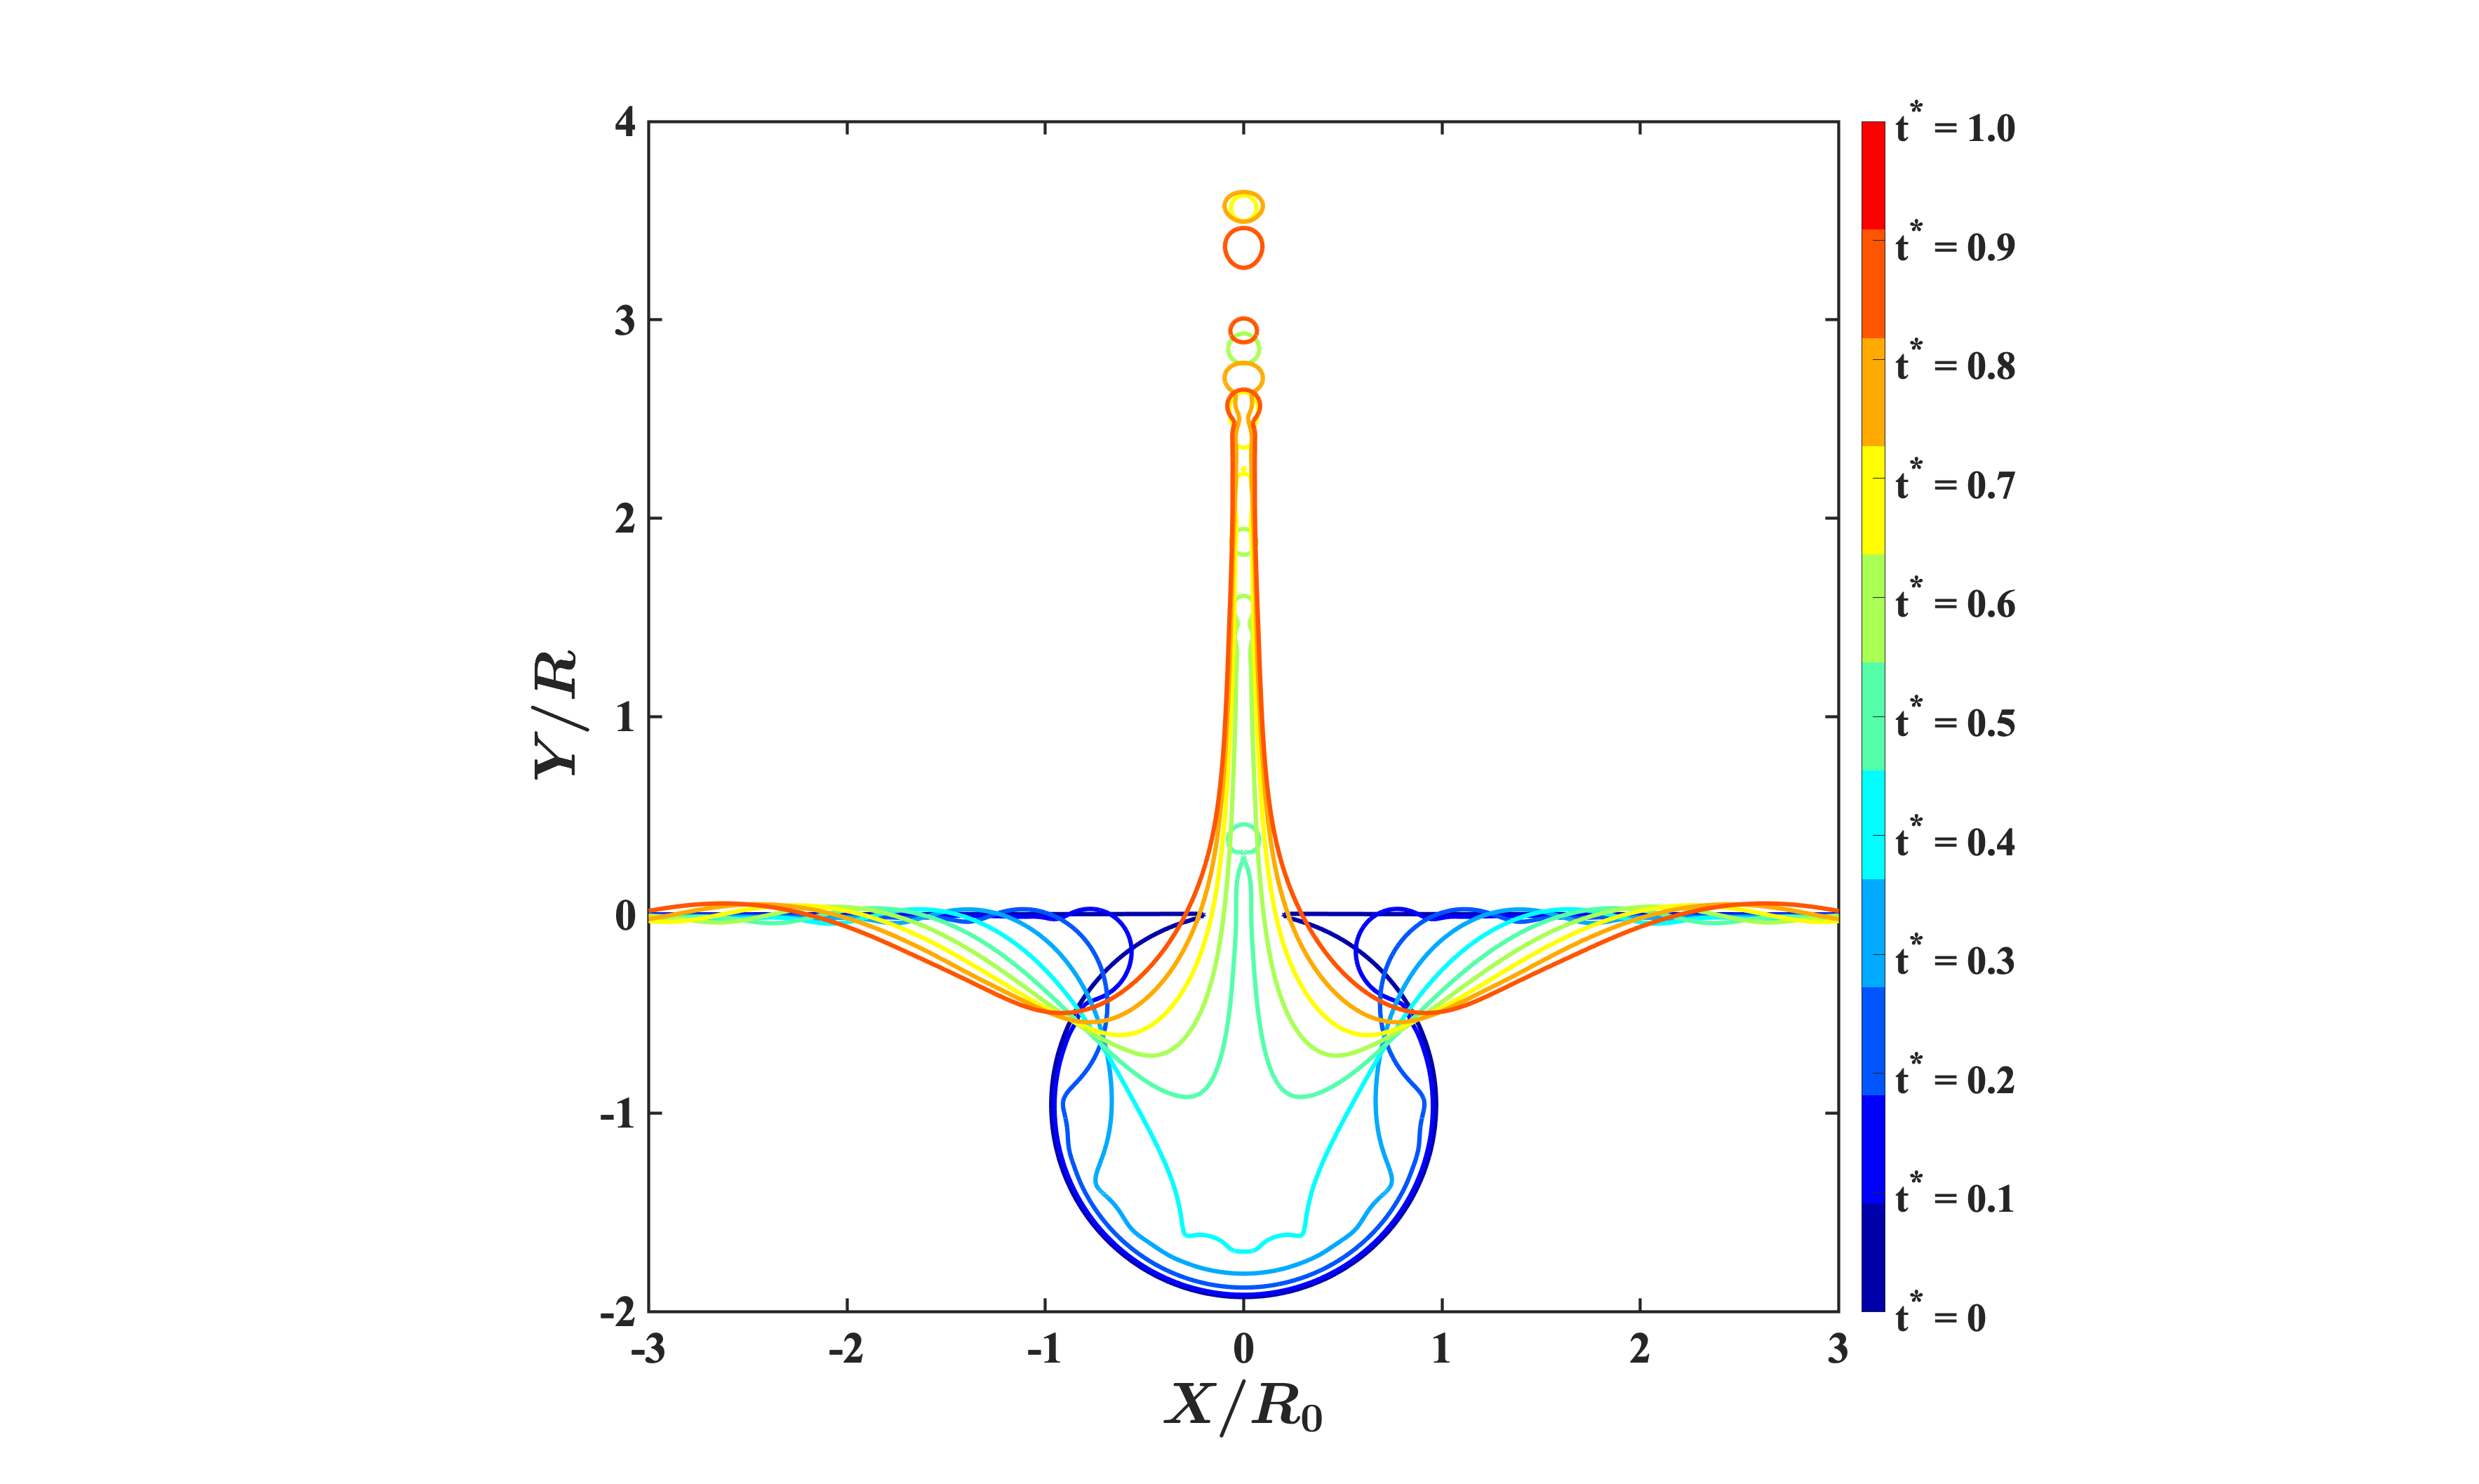
\includegraphics[width=\textwidth]{interface.eps}
 \caption{Collapse of the bubble cavity and interaction of capillary waves}
 \label{Figure::Waves}
\end{center}
\end{figure}
\section*{What you will do and what you will learn?}
% The project will focus on the following:
\begin{enumerate}
\item You will learn about the fundamental fluid mechanics of two-phase flows.
\item You will learn the science of rheology.
\item You will learn the freeware code \href{http://basilisk.fr}{Basilisk C} to simulate fluid dynamics problems.
%\item Validation of the numerical model using the scaling laws available in the literature for the collapse of air bubble cavity in Newtonian fluid pool \citep{duchemin2002jet}.
%\item Implementation and validation of the generalized Newtonian fluid viscosity model to the free-code \href{http://basilisk.fr}{Basilisk C }.
%\item Studying the effects of a Viscoplastic liquid medium on the bursting of bubbles at the interface.
%\item Understanding the dependence of the liquid's viscoplasticity on the proposed scaling laws.
\end{enumerate}
If you have any questions, fell to contact \href{mailto:v.sanjay@utwente.nl}{Vatsal} or \href{mailto:m.jalaal@utwente.nl}{Mazi} (details below).
\begin{center}
\begin{tabular}{|l|l|l|l|}
\hline \textbf{Supervision} & \textbf{E-mail} & \textbf{Office} \\
\hline Vatsal Sanjay & \href{mailto:v.sanjay@utwente.nl}{v.sanjay@utwente.nl} & Meander 212 \\
\hline Dr. Maziyar (Mazi) Jalaal   & \href{mailto:m.jalaal@utwente.nl}{m.jalaal@utwente.nl}& Meander 208 \\
\hline Prof. D. Lohse & \href{mailto:d.lohse@utwente.nl}{d.lohse@utwente.nl} & Meander 261  \\
\hline
\end{tabular}
\end{center}
\printbibliography
\end{document}
